% Shared standalone design for the editable figure reconstructions.
\documentclass[tikz,border=5pt,10pt]{standalone}
\usepackage[T1]{fontenc}
\usepackage[utf8]{inputenc}
\usepackage{newpxtext,newpxmath}
\usepackage[scaled=.94]{sourcesanspro}
\usepackage{pgfplots}
\pgfplotsset{compat=1.18}
\usetikzlibrary{arrows.meta,calc,positioning,decorations.pathreplacing,
  decorations.markings,patterns,matrix,shapes.geometric,fit,backgrounds,
  intersections,angles,quotes}
\definecolor{ink}{HTML}{203746}
\definecolor{accent}{HTML}{146C78}
\definecolor{muted}{HTML}{667780}
\definecolor{signalred}{HTML}{B94B44}
\color{ink}
\tikzset{>=Latex,line width=.8pt,
  every node/.style={font=\small},
  axis/.style={->,draw=muted,line width=.5pt},
  guide/.style={draw=muted,dashed,line width=.45pt},
  curve/.style={draw=accent,line width=1pt},
  marker/.style={circle,fill=accent,inner sep=1.5pt},
  labelbox/.style={fill=white,inner sep=2pt}}

\begin{document}
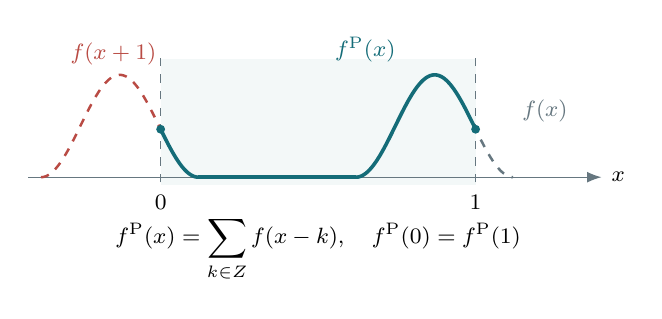
\begin{tikzpicture}[x=4cm,y=1.3cm,every node/.style={font=\footnotesize}]
% Illustrative compact bump: f(x)=cos^2(2 pi (x-.87)) for |x-.87|<=.25,
% zero otherwise. On [0,1] only f(x) and f(x+1) can contribute.
\fill[accent!5] (0,-.08) rectangle(1,1.15);
\draw[axis] (-.42,0)--(1.4,0) node[right] {$x$};
\draw[guide] (0,-.05)--(0,1.23) (1,-.05)--(1,1.23);
\draw[muted,dashed,line width=.9pt,domain=.62:1.12,samples=101] plot (\x,{cos(360*(\x-.87))^2});
\draw[signalred,dashed,line width=.9pt,domain=-.38:.12,samples=101] plot (\x,{cos(360*(\x+.13))^2});
\draw[curve,line width=1.3pt,domain=0:.12,samples=51] plot (\x,{cos(360*(\x+.13))^2});
\draw[curve,line width=1.3pt] (.12,0)--(.62,0);
\draw[curve,line width=1.3pt,domain=.62:1,samples=101] plot (\x,{cos(360*(\x-.87))^2});
\node[muted] at (1.22,.65) {$f(x)$};\node[signalred] at (-.15,1.2) {$f(x+1)$};
\node[accent] at (.65,1.25) {$f^{\mathrm P}(x)$};
\foreach \x in {0,1} {\node[below] at (\x,-.08) {$\x$};\fill[accent] (\x,{cos(360*.13)^2}) circle(1.6pt);}
\node at (.5,-.7) {$\displaystyle f^{\mathrm P}(x)=\sum_{k\in\mathbb Z}f(x-k),\quad f^{\mathrm P}(0)=f^{\mathrm P}(1)$};
\end{tikzpicture}
\end{document}
